\documentclass[12pt]{article}
\usepackage[a4paper, margin=0.7in]{geometry}
\usepackage[utf8]{inputenc}
\usepackage[hidelinks, colorlinks=false]{hyperref}
\usepackage{graphicx}
\usepackage{booktabs}
\usepackage{amsmath}
\usepackage{caption}
\usepackage{float}
\usepackage{longtable}
\usepackage{ragged2e}
\usepackage{setspace}
\usepackage[backend=biber, style=apa, natbib=true]{biblatex}
\addbibresource{references.bib} 
\onehalfspacing


\title{Online Appendix for ``Complex survival: institutional overlap and the different forms of international organization termination"}
\author{João Pedro Martins}
\date{}


\begin{document}

\maketitle

\tableofcontents
\newpage

\section*{Introduction to the Online Appendix}
\addcontentsline{toc}{section}{Introduction to the Online Appendix}
This document contains supplementary materials for my paper ``Complex survival: institutional overlap and the different forms of international organization termination." 

It includes additional analyses, robustness checks, and detailed methodological discussions that complement the main paper.

\section*{Discussion on survival analysis and competing risks}
\addcontentsline{toc}{section}{Discussion on survival analysis and competing risks}

Here, I present a brief explanation of the quantities of interest in survival analysis and competing risks analysis. For political science, Box-Steffensmeier and Jones (\citeyear{box2004event}) remains the most relevant introduction. Recently, Flores (\citeyear{flores2022survival}) published a new guide on survival analysis for social scientists.\footnote{I'm particularly indebted to Prof. Alex Flores for gently sending me the paperback edition of his book. Without his act of pure kindness and academic commitment, my process of learning these methods would have been significantly harder.} His book is a very important contribution to this area, bringing to political science some of the advances in survival analysis that occurred in the two-decade interval between his book and Box-Steffensmeier and Jones'.

To elaborate my explanation below on competing risks analysis, I build upon the works of Austin et al. (\citeyear{austin2016introduction}), Flores (\citeyear{flores2022survival}), Geskus (\citeyear{geskus2024competing}), Kalbfleisch and Schaubel (\citeyear{kalbfleisch2023fifty}), Latouche et al. (\citeyear{latouche2013competing}), Putter et al. (\citeyear{putter2007tutorial}), Putter et al. (\cite{putter2020relation}), and Therneau et al. (\citeyear{therneau2024multi}). For better flow in the explanation of these issues, I chose to explicitly mention their works here rather than in the body of the text. All analyses and explanations come from these works.

One of the most important quantities of interest in survival analysis is the hazard rate ($\lambda(t)$). The hazard rate is the conditional probability of failure, i.e., the instantaneous rate of occurrence of the event of interest. In simple survival analysis, in the absence of competing risks, the hazard rate is defined as: 

\begin{equation}
\lambda(t) = \lim_{\Delta t \to 0} \frac{P(t \leq T < t + \Delta t \mid T \geq t)}{\Delta t} = \frac{f(t)}{S(t)}
\end{equation}

Here $f(t)$ is the probability density function of the variable $T$, and $S(t)$ is the survival function ($S(t) = 1 - F(t) = \Pr(T \geq t)$). In this simple case, for the Cox proportional hazards model, we have the following:


\begin{equation}
\lambda(t \mid Z) = \lambda_0(t) \exp(\beta^\top Z)
\end{equation}

where \(\beta\) is a vector of regression coefficients, \(Z\) is a vector of covariates, and \(\lambda_0(t)\) represents the baseline hazard.

Before really entering into the discussion of the two approaches to competing risks, it is important to define one of the main quantities of interest here, the cumulative incidence function (CIF). The CIF for the \(k\)-th cause is defined as:

\begin{equation}
I_k(t) = \Pr(T \leq t, D = k),
\end{equation}

where \(D\) is a variable denoting the type of event. It is basically the probability of failing from a given cause \(k\) before time \(t\). The cumulative incidence is a special case of the Aalen-Johansen estimator, which is why it is possible to use this estimator to calculate it. We will return to the discussion about the CIF right back, but now it is important to stress the differences in the types of hazard functions. 

In the presence of competing risks, where there are multiple events of interest, there are two possible approaches to the hazard functions: the cause-specific hazard function and the subdistribution hazard function. The cause-specific hazard function is defined as follows:

\begin{equation}
\lambda_k(t) = \lim_{\Delta t \to 0} \frac{\Pr(t \leq T < t + \Delta t, D = k \mid T \geq t)}{\Delta t}
\end{equation}

where  \(\lambda_k(t)\) is the cause-specific hazard function for cause \(k\). Here, when an individual experiences a competing event, he leaves the risk set. Therefore, in the cause-specific approach, the hazard function is the instantaneous rate of occurrence of the \(k\)-th event in individuals who have not yet experienced any event. In a Cox regression, in this case, individuals who experience an event different from k are treated as censored. Importantly, each cause is assumed to have its own baseline hazard function. In terms of cause-specific hazards, the CIF is expressed as follows:

\begin{equation}
I_k(t) = \int_0^t \lambda_k(s) S(s) \, ds
\end{equation}

Here, events from causes other than \(k\) are treated as censored. Therefore, the naive Kaplan–Meier estimate is given by:

\begin{equation}
1 - S_k(t) = \int_0^t \lambda_k(s) S_k(s) \, ds
\end{equation} 

Comparing this with the immediately anterior equation we see an important difference. \( S(s) \) is replaced by \( S_k(s) \). Since \( S(t) \leq S_k(t) \), we have \( I_k(t) \leq 1 - S_k(t) \). Here resides precisely that bias described in the first paragraph of section 5.2 of the paper. The artificial censoring of units that do not fail for the right reason causes that bias, which makes the Kaplan-Meier estimator inappropriate in the presence of competing risks. 

However, the cause-specific approach does not allow for the estimation of the covariate effects on the CIFs. This is because the CIF for cause \(k\) not only depends on the hazard of \(k\), but also on the hazards of all other causes. In some cases, the direction of the relationship on the cumulative scale can even reverse. The proposed solution for this problem was given by Fine and Gray in their 1999 paper. There they introduce the subdistribution hazard function, which has the following format:

\begin{equation}
\gamma_k(t)=\lim_{\Delta t \to 0} \frac{\text{Prob}(t \leq T \leq t + \Delta t, D = k | T \geq t \cup (T \leq t \cap K \neq k))}{\Delta t}
\end{equation}

Different from the cause-specific approach, it is possible to see that the risk set includes those who have not experienced an event yet and those who have previously experienced a competing event). The main difficulty here is that the occurrence of \( D = k \) precludes the occurrence of any other \( D \neq k \). The solution from Fine and Gray involves defining the distribution function for the improper random variable \( T^* \) as follows:

\begin{equation}
T^* = I(D = k)T + I(D \neq k)\infty.
\end{equation}

As discussed earlier, the hazard rate is the ratio \( f(t) / S(t) \) and both can be expressed as functions of the CIF. Therefore:

\begin{equation}
\gamma_k(t) = -\frac{d \log(1 - I_k(t))}{dt}
\end{equation}

The two models presented here have advantages and disadvantages, and a researcher must be aware of these differences when interpreting the results. The cause-specific approach, which is the multi-state approach for competing risks, is more straightforward in terms of estimation and interpretation. It is fundamental to distinguish the interpretation about the incidence rate and the hazard rate. If one is aware that it does not estimate the covariate effect on the CIFs and explicitly explains that in the discussion, this is perhaps the most immediate choice regarding competing risks for political science.

Multi-state survival models are starting to become more popular in political science (\cite{metzger2016surviving}). However, the use of competing risks models in political science is still somewhat rare, especially in the study of international organizations. A brief search in Google Scholar reported very few articles in this area that use these approaches and provide a comprehensive discussion of these methods in international relations.

Most of the literature I used to write this section is medical literature and is concerned with medical problems, which are different from political science problems and research questions. However, their insights about which approach is more appropriate to which question are still relevant here. This literature tends to defend that cause-specific hazards are more appropriate for addressing epidemiological questions of etiology and subdistribution hazards for clinical prediction models. Moreover, when the focus is on understanding the underlying mechanisms of a given process, this medical literature tends to favor cause-specific hazards.

Perhaps for political science, the inferential\footnote{The discussion about causality, even in the context of competing risks in medical literature, is really complex and exceeds the scope of our discussion here.} question is the most important. Here, the standard procedure established by Latouche et al. (\citeyear{latouche2013competing}) can be adapted and used in political science for a more appropriate analysis of competing risks. Some of the most important recommendations are: 

\begin{itemize}
    \item Using a distinct terminology for each model of the hazard ratio, namely cause-specific hazards for the Cox model and subdistribution hazards for the Fine and Gray model;
    \item Reporting all the cause-specific hazards;
    \item Reporting the subdistribution hazard for the event of interest and the subdistribution hazard for the competing event;
    \item Presenting the results in a unified interpretation, so as to connect and reconcile results from the two sets of models;
    \item Explicitly checking the proportional hazards assumption for the Cox and Fine and Gray models.
\end{itemize}

In my article I tried to follow these recommendations, with the small difference that I reported the coefficients rather than the hazard ratios, which appears to be a more straightforward approach for a political science audience. Jones and Metzger (\citeyear{jones2019different}), while giving recommendations for duration models in a broader sense, also provide an important framework for political scientists interested in these discussions. 






\newpage
\section*{Table A1: Descriptive statistics}
\addcontentsline{toc}{section}{Table A1: Descriptive statistics}

\begin{table}[!htbp] \centering 
  \label{} 
\begin{tabular}{@{\extracolsep{5pt}} ccccccc} 
\\[-1.8ex]\hline 
\hline \\[-1.8ex] 
 Variable & Mean & SD & Median & Min & Max \\ 
\hline \\[-1.8ex] 
IO death & $0.010$ & $0.101$ & $0$ & $0$ & $1$ \\ 
Duration & $27.884$ & $25.249$ & $21$ & $1$ & $200$ \\ 
Institutional overlap & $0.023$ & $0.026$ & $0.015$ & $0$ & $0.274$ \\ 
Number of members & $29.190$ & $37.619$ & $16$ & $1$ & $193$ \\ 
Number of living IOs & $236.502$ & $106.035$ & $286$ & $0$ & $336$ \\ 
Policy scope & $1.841$ & $1.062$ & $2$ & $0$ & $8$ \\ 
Governance mandates & $3.538$ & $1.572$ & $3$ & $0$ & $8$ \\ 
Institutionalization & $3.183$ & $1.497$ & $3$ & $0$ & $6$ \\ 
\hline \\[-1.8ex] 
\end{tabular} 
\end{table} 

\newpage
\section*{Table A2: IOs that ended due to contract-based terminations}
\addcontentsline{toc}{section}{Table A2: IOs that ended due to contract-based terminations}


\begin{longtable}{lp{5.5cm}ccc}
\caption*{} \\
\hline
\textbf{Acronym} & \textbf{Organization Name} & \textbf{Birth} & \textbf{Death} & \textbf{Type} \\
\hline
\endfirsthead

\hline
\textbf{Acronym} & \textbf{Organization Name} & \textbf{Birth} & \textbf{Death} & \textbf{Type} \\
\hline
\endhead

\hline
\multicolumn{5}{r}{\textit{Continued}} \\
\endfoot

\hline
\endlastfoot

AMSC & {\RaggedRight\hyphenpenalty=10000 African and Malagasy Sugar Council} & 1966 & 1977 & Dissolution \\
ACI & {\RaggedRight\hyphenpenalty=10000 African Cultural Institute} & 1971 & 1999 & Dissolution \\
AMCO & {\RaggedRight\hyphenpenalty=10000 African Malagasy Coffee Organization} & 1960 & 2007 & Dissolution \\
OCAM & {\RaggedRight\hyphenpenalty=10000 Afro-Malagasy Union} & 1961 & 1985 & Dissolution \\
AITIC & {\RaggedRight\hyphenpenalty=10000 Agency for International Trade Information and Cooperation} & 2004 & 2011 & Dissolution \\
ASPAC & {\RaggedRight\hyphenpenalty=10000 Asian and Pacific Council} & 1966 & 1973 & Dissolution \\
Corg & {\RaggedRight\hyphenpenalty=10000 Caribbean Organization} & 1960 & 1965 & Dissolution \\
CAMSF & {\RaggedRight\hyphenpenalty=10000 Central American Monetary Stabilization Fund} & 1969 & 1991 & Dissolution \\
CARII & {\RaggedRight\hyphenpenalty=10000 Central American Research Institute for Industry} & 1956 & 1997 & Dissolution \\
CPAB & {\RaggedRight\hyphenpenalty=10000 Central Pan American Bureau of Eugenics and Homiculture} & 1927 & 1949 & Dissolution \\
CENTO & {\RaggedRight\hyphenpenalty=10000 Central Treaty Organization} & 1955 & 1979 & Dissolution \\
CIFC & {\RaggedRight\hyphenpenalty=10000 Commission for International Financial Control in Macedonia} & 1905 & 1914 & Dissolution \\
CHSTEA & {\RaggedRight\hyphenpenalty=10000 Conference of Heads of State of Equatorial Africa} & 1960 & 1968 & Dissolution \\
CMEA & {\RaggedRight\hyphenpenalty=10000 Council for Mutual Economic Aid} & 1949 & 1991 & Dissolution \\
EACM & {\RaggedRight\hyphenpenalty=10000 East African Common Market} & 1967 & 1977 & Dissolution \\
EMB & {\RaggedRight\hyphenpenalty=10000 Empire Marketing Board} & 1926 & 1933 & Dissolution \\
ECCD & {\RaggedRight\hyphenpenalty=10000 European Commission for Control of the Danube} & 1856 & 1939 & Dissolution \\
ECCPIF & {\RaggedRight\hyphenpenalty=10000 European Company for Chemical Processing of Irradiated Fuels} & 1957 & 1984 & Dissolution \\
FEC & {\RaggedRight\hyphenpenalty=10000 Far East Commission} & 1945 & 1951 & Dissolution \\
GLACSEC & {\RaggedRight\hyphenpenalty=10000 Group of Latin American and Caribbean Sugar Exporting Countries} & 1974 & 2001 & Dissolution \\
G3 & {\RaggedRight\hyphenpenalty=10000 Group of Three} & 1995 & 2006 & Dissolution \\
GCRSNC & {\RaggedRight\hyphenpenalty=10000 Guidance Committee for Road Safety in Nordic Countries} & 1993 & 1999 & Dissolution \\
IARA & {\RaggedRight\hyphenpenalty=10000 Inter-Allied Reparation Agency} & 1946 & 1955 & Dissolution \\
IARHC & {\RaggedRight\hyphenpenalty=10000 Inter-Allied Rhineland High Commission} & 1919 & 1934 & Expiry \\
IAII & {\RaggedRight\hyphenpenalty=10000 Inter-American Indian Institute} & 1940 & 1953 & Dissolution \\
IARadiO & {\RaggedRight\hyphenpenalty=10000 Inter-American Radio Office} & 1937 & 1963 & Dissolution \\
IATB & {\RaggedRight\hyphenpenalty=10000 Inter-American Trademark Bureau} & 1917 & 1944 & Dissolution \\
IBI & {\RaggedRight\hyphenpenalty=10000 Intergovernmental Bureau for Informatics} & 1974 & 1991 & Dissolution \\
IAMLO & {\RaggedRight\hyphenpenalty=10000 International African Migratory Locust Organization} & 1952 & 1985 & Dissolution \\
IATSJ & {\RaggedRight\hyphenpenalty=10000 International Arbitration Tribunal at San Jose} & 1907 & 1916 & Dissolution \\
IAS & {\RaggedRight\hyphenpenalty=10000 International Association of Seismology} & 1903 & 1922 & Dissolution \\
IARuhr & {\RaggedRight\hyphenpenalty=10000 International Authority for the Ruhr} & 1949 & 1953 & Dissolution \\
IBCS & {\RaggedRight\hyphenpenalty=10000 International Bureau of Commercial Statistics} & 1913 & 1935 & Dissolution \\
ICCSLT & {\RaggedRight\hyphenpenalty=10000 International Commission of the Cape Spartel Light in Tangier} & 1865 & 1958 & Dissolution \\
ICTM & {\RaggedRight\hyphenpenalty=10000 International Commission on the Teaching of Mathematics} & 1908 & 1939 & Dissolution \\
IJO & {\RaggedRight\hyphenpenalty=10000 International Jute Organization} & 1984 & 2001 & Expiry \\
IMBSlav & {\RaggedRight\hyphenpenalty=10000 International Maritime Bureau Against the Slave Trade} & 1890 & 1909 & Dissolution \\
INRO & {\RaggedRight\hyphenpenalty=10000 International Natural Rubber Organization} & 1980 & 1999 & Expiry \\
IRO & {\RaggedRight\hyphenpenalty=10000 International Refugee Organization} & 1946 & 1952 & Dissolution \\
IRU & {\RaggedRight\hyphenpenalty=10000 International Relief Union} & 1927 & 1968 & Dissolution \\
ITC & {\RaggedRight\hyphenpenalty=10000 International Tin Council} & 1956 & 1990 & Dissolution \\
IWSG & {\RaggedRight\hyphenpenalty=10000 International Wool Study Group} & 1947 & 1992 & Dissolution \\
LoN & {\RaggedRight\hyphenpenalty=10000 League of Nations} & 1919 & 1945 & Dissolution \\
NERC & {\RaggedRight\hyphenpenalty=10000 Nordic Economic Research Council} & 1979 & 1996 & Dissolution \\
NTSC & {\RaggedRight\hyphenpenalty=10000 Nordic Telecommunications Satellite Council} & 1965 & 1986 & Dissolution \\
NPFSC & {\RaggedRight\hyphenpenalty=10000 North Pacific Fur Seal Commission} & 1958 & 1988 & Dissolution \\
SEATO & {\RaggedRight\hyphenpenalty=10000 Southeast Asia Treaty Organization} & 1954 & 1977 & Dissolution \\
SAAFA & {\RaggedRight\hyphenpenalty=10000 Special Arab Aid Fund for Africa} & 1974 & 1977 & Dissolution \\
SCH & {\RaggedRight\hyphenpenalty=10000 Superior Council of Health} & 1838 & 1914 & Dissolution \\
TCRMG & {\RaggedRight\hyphenpenalty=10000 Tripartite Commission for the Restitution of Monetary Gold} & 1946 & 1998 & Dissolution \\
UKDWD & {\RaggedRight\hyphenpenalty=10000 United Kingdom--Dominion Wool Disposals} & 1945 & 1953 & Dissolution \\
WPact & {\RaggedRight\hyphenpenalty=10000 Warsaw Treaty Organization} & 1955 & 1991 & Dissolution \\
WEU & {\RaggedRight\hyphenpenalty=10000 Western European Union} & 1955 & 2011 & Dissolution \\
\end{longtable}

\newpage
\section*{Table A3: IOs that ended due to transformation-based terminations}
\addcontentsline{toc}{section}{Table A3: IOs that ended due to transformation-based terminations}

\begin{longtable}{lp{5.5cm}ccc}
\caption*{} \\
\hline
\textbf{Acronym} & \textbf{Organization Name} & \textbf{Birth} & \textbf{Death} & \textbf{Type} \\
\hline
\endfirsthead

\hline
\textbf{Acronym} & \textbf{Organization Name} & \textbf{Birth} & \textbf{Death} & \textbf{Type} \\
\hline
\endhead

\hline
\multicolumn{5}{r}{\textit{Continued}} \\
\endfoot

\hline
\endlastfoot

APTU & {\RaggedRight\hyphenpenalty=10000 African Postal and Telecommunications Union} & 1935 & 1965 & Succession \\
AMIPO & {\RaggedRight\hyphenpenalty=10000 Afro-Malagasy Industrial Property Office} & 1962 & 1975 & Succession \\
AMPTU & {\RaggedRight\hyphenpenalty=10000 Afro-Malagasy Postal and Telecommunications Union} & 1961 & 1996 & Succession \\
ACCT & {\RaggedRight\hyphenpenalty=10000 Agence de La Francophonie} & 1970 & 2005 & Succession \\
AOMR & {\RaggedRight\hyphenpenalty=10000 Arab Organization for Mineral Resources} & 1979 & 1991 & Merger \\
AIDC & {\RaggedRight\hyphenpenalty=10000 Asian Industrial Development Council} & 1966 & 1974 & Merger \\
ABEPSEAC & {\RaggedRight\hyphenpenalty=10000 Association between the European Economic Community and Partner States} & 1968 & 1975 & Succession \\
BIISEF & {\RaggedRight\hyphenpenalty=10000 Banque internationale d'information sur les Etats francophones} & 1986 & 1996 & Absorption \\
CComm & {\RaggedRight\hyphenpenalty=10000 Caribbean Commission} & 1946 & 1959 & Succession \\
CARIFTA & {\RaggedRight\hyphenpenalty=10000 Caribbean Free Trade Association} & 1966 & 1973 & Succession \\
UDEAC & {\RaggedRight\hyphenpenalty=10000 Central African Customs and Economic Union} & 1964 & 1994 & Succession \\
CACB & {\RaggedRight\hyphenpenalty=10000 Central American Coffee Board} & 1975 & 1979 & Succession \\
CAECC & {\RaggedRight\hyphenpenalty=10000 Central Asian Economic Community} & 1994 & 2006 & Absorption \\
CBI & {\RaggedRight\hyphenpenalty=10000 Central Bureau for the International Map of the World} & 1909 & 1953 & Merger \\
CTCAf & {\RaggedRight\hyphenpenalty=10000 Commission for Technical Cooperation in Africa South of the Sahara} & 1950 & 1965 & Succession \\
CAARC & {\RaggedRight\hyphenpenalty=10000 Commonwealth Advisory Aeronautical Research Council} & 1946 & 1993 & Absorption \\
ComAB & {\RaggedRight\hyphenpenalty=10000 Commonwealth Agricultural Bureau} & 1929 & 1985 & Succession \\
CEC & {\RaggedRight\hyphenpenalty=10000 Commonwealth Economic Committee} & 1925 & 1967 & Absorption \\
CELC & {\RaggedRight\hyphenpenalty=10000 Commonwealth Education Liaison Committee} & 1960 & 1967 & Absorption \\
CAMRSD & {\RaggedRight\hyphenpenalty=10000 Conference of African Ministers Responsible for Sustainable Development} & 1993 & 1997 & Succession \\
CMAEC & {\RaggedRight\hyphenpenalty=10000 Council of Ministers for Asian Economic Cooperation} & 1968 & 1971 & Succession \\
EACSO & {\RaggedRight\hyphenpenalty=10000 East African Common Services Organization} & 1961 & 1967 & Succession \\
ECCM & {\RaggedRight\hyphenpenalty=10000 East Caribbean Common Market} & 1968 & 1981 & Absorption \\
ECCA & {\RaggedRight\hyphenpenalty=10000 Eastern Caribbean Currency Area} & 1979 & 1983 & Succession \\
ECSC & {\RaggedRight\hyphenpenalty=10000 European Coal and Steel Community} & 1952 & 1992 & Absorption \\
EUROMET & {\RaggedRight\hyphenpenalty=10000 European Collaboration on Measurement Standards} & 1987 & 2007 & Succession \\
EFCC & {\RaggedRight\hyphenpenalty=10000 European Food Code Council} & 1958 & 1965 & Absorption \\
EEC & {\RaggedRight\hyphenpenalty=10000 European Economic Community} & 1958 & 1992 & Absorption \\
EMI & {\RaggedRight\hyphenpenalty=10000 European Monetary Institute} & 1994 & 1998 & Succession \\
EPU & {\RaggedRight\hyphenpenalty=10000 European Payments Union} & 1950 & 1958 & Succession \\
EPA & {\RaggedRight\hyphenpenalty=10000 European Productivity Agency} & 1953 & 1961 & Absorption \\
ESRO & {\RaggedRight\hyphenpenalty=10000 European Space Research Organization} & 1964 & 1975 & Merger \\
ELDO & {\RaggedRight\hyphenpenalty=10000 European Space Vehicle Launcher Development Organization} & 1964 & 1975 & Merger \\
GATT & {\RaggedRight\hyphenpenalty=10000 General Agreement on Tariffs and Trade} & 1948 & 1995 & Succession \\
SCHENGEN & {\RaggedRight\hyphenpenalty=10000 Group of Schengen} & 1985 & 1999 & Absorption \\
IDC & {\RaggedRight\hyphenpenalty=10000 Imperial Defense Committee} & 1920 & 1946 & Absorption \\
IIE & {\RaggedRight\hyphenpenalty=10000 Imperial Institute of Entomology} & 1920 & 1933 & Succession \\
IMI & {\RaggedRight\hyphenpenalty=10000 Imperial Mycological Institute} & 1920 & 1933 & Succession \\
IACS & {\RaggedRight\hyphenpenalty=10000 Inter-African Committee on Statistics} & 1954 & 1965 & Succession \\
IAPhy & {\RaggedRight\hyphenpenalty=10000 Inter-African Phytosanitary Convention} & 1954 & 1960 & Absorption \\
IACB & {\RaggedRight\hyphenpenalty=10000 Inter-American Coffee Board} & 1940 & 1948 & Succession \\
IACW & {\RaggedRight\hyphenpenalty=10000 Inter-American Commission of Women} & 1928 & 1965 & Absorption \\
IGCC & {\RaggedRight\hyphenpenalty=10000 Intergovernmental Copyright Committee} & 1952 & 1971 & Absorption \\
ICCILMB & {\RaggedRight\hyphenpenalty=10000 Interim Committee for Coordination of Investigations of the Lower Mekong Basin} & 1978 & 1995 & Succession \\
IBIER & {\RaggedRight\hyphenpenalty=10000 International Bureau for Information and Enquiries regarding Relief} & 1907 & 1921 & Absorption \\
IBE & {\RaggedRight\hyphenpenalty=10000 International Bureau of Education} & 1929 & 1969 & Absorption \\
ICNWAF & {\RaggedRight\hyphenpenalty=10000 International Commission for the Northwest Atlantic Fisheries} & 1949 & 1978 & Succession \\
IIA & {\RaggedRight\hyphenpenalty=10000 International Institute of Agriculture} & 1905 & 1945 & Succession \\
IMC & {\RaggedRight\hyphenpenalty=10000 International Moselle Company} & 1956 & 1987 & Succession \\
INPFC & {\RaggedRight\hyphenpenalty=10000 International North Pacific Fisheries Commission} & 1952 & 1992 & Succession \\
IOPH & {\RaggedRight\hyphenpenalty=10000 International Office of Public Hygiene} & 1907 & 1946 & Succession \\
IPI & {\RaggedRight\hyphenpenalty=10000 International Patent Institute} & 1947 & 1977 & Absorption \\
IPentC & {\RaggedRight\hyphenpenalty=10000 International Penitentiary Commission} & 1875 & 1951 & Absorption \\
IRLCS & {\RaggedRight\hyphenpenalty=10000 International Red Locust Control Service} & 1949 & 1970 & Succession \\
ISuC & {\RaggedRight\hyphenpenalty=10000 International Sugar Council} & 1937 & 1967 & Succession \\
ITCLE & {\RaggedRight\hyphenpenalty=10000 International Technical Committee of Legal Experts on Air Questions} & 1926 & 1941 & Succession \\
INTELSAT & {\RaggedRight\hyphenpenalty=10000 International Telecommunications Satellite Organization} & 1964 & 2001 & Succession \\
ITCC & {\RaggedRight\hyphenpenalty=10000 International Telegraph Consultative Committee} & 1925 & 1956 & Merger \\
IVWO & {\RaggedRight\hyphenpenalty=10000 International Wine Office} & 1924 & 2003 & Succession \\
IOATHRE & {\RaggedRight\hyphenpenalty=10000 Inter-State Organization for Advanced Technicians of Hydraulics} & 1972 & 2004 & Merger \\
LAFTA & {\RaggedRight\hyphenpenalty=10000 Latin American Free Trade Association} & 1961 & 1980 & Succession \\
NCRR & {\RaggedRight\hyphenpenalty=10000 Nordic Council for Reindeer Research} & 1980 & 1992 & Absorption \\
OAU & {\RaggedRight\hyphenpenalty=10000 Organization for African Unity} & 1963 & 2002 & Succession \\
OEEC & {\RaggedRight\hyphenpenalty=10000 Organization for European Economic Cooperation} & 1948 & 1961 & Succession \\
OMDKR & {\RaggedRight\hyphenpenalty=10000 Organization for the Management and Development of the Kagera River} & 1977 & 2000 & Absorption \\
OCAS & {\RaggedRight\hyphenpenalty=10000 Organization of Central American States} & 1951 & 1991 & Succession \\
OSLO & {\RaggedRight\hyphenpenalty=10000 Oslo Commission} & 1972 & 1998 & Succession \\
PC & {\RaggedRight\hyphenpenalty=10000 Paris Commission} & 1977 & 1998 & Succession \\
PAHC & {\RaggedRight\hyphenpenalty=10000 Permanent Association of Pan American Highway Congresses} & 1939 & 1952 & Absorption \\
PIBAC & {\RaggedRight\hyphenpenalty=10000 Permanent International Bureau of Analytical Chemistry} & 1923 & 1934 & Succession \\
PTASEA & {\RaggedRight\hyphenpenalty=10000 Preferential Trade Agreement for Southern \& Eastern Africa} & 1981 & 1994 & Succession \\
RadioU & {\RaggedRight\hyphenpenalty=10000 Radiotelegraph Union} & 1906 & 1926 & Merger \\
SCAf & {\RaggedRight\hyphenpenalty=10000 Scientific Council for Africa South of the Sahara} & 1950 & 1965 & Merger \\
SARTC & {\RaggedRight\hyphenpenalty=10000 Southern Africa Regional Tourism Council} & 1973 & 1996 & Succession \\
SADCC & {\RaggedRight\hyphenpenalty=10000 Southern African Development Coordination Conference} & 1980 & 1992 & Succession \\
UIUCV & {\RaggedRight\hyphenpenalty=10000 Union for the International Use of Carriages and Vans} & 1923 & 1979 & Succession \\
UMAC & {\RaggedRight\hyphenpenalty=10000 Union montaire de l'Afrique centrale} & 1972 & 1994 & Absorption \\
CEAO & {\RaggedRight\hyphenpenalty=10000 West African Economic Community} & 1960 & 1994 & Succession \\
WAHC & {\RaggedRight\hyphenpenalty=10000 West African Health Community} & 1972 & 1987 & Succession \\
UMOA & {\RaggedRight\hyphenpenalty=10000 West African Monetary Union} & 1962 & 1994 & Succession \\
\end{longtable}

\newpage
\section*{Table A4: IOs that ended due to inertia-based terminations}
\addcontentsline{toc}{section}{Table A4: IOs that ended due to inertia-based terminations}

\begin{longtable}{lp{5.5cm}ccc}
\caption*{} \\
\hline
\textbf{Acronym} & \textbf{Organization Name} & \textbf{Birth} & \textbf{Death} & \textbf{Type} \\
\hline
\endfirsthead

\hline
\textbf{Acronym} & \textbf{Organization Name} & \textbf{Birth} & \textbf{Death} & \textbf{Type} \\
\hline
\endhead

\hline
\multicolumn{5}{r}{\textit{Continued}} \\
\endfoot

\hline
\endlastfoot

ASCBC & {\RaggedRight\hyphenpenalty=10000 African Standing Conference on Bibliographic Control} & 1978 & 2000 & Desuetude \\
ACDT & {\RaggedRight\hyphenpenalty=10000 American Committee on Dependent Territories} & 1948 & 1956 & Desuetude \\
ACML & {\RaggedRight\hyphenpenalty=10000 Arab Centre for Medical Literature} & 1983 & 2000 & Desuetude \\
ACC & {\RaggedRight\hyphenpenalty=10000 Arab Cooperation Council} & 1989 & 1990 & Desuetude \\
AIOEC & {\RaggedRight\hyphenpenalty=10000 Association of Iron Ore Exporting Countries} & 1975 & 1998 & Desuetude \\
ATPC & {\RaggedRight\hyphenpenalty=10000 Association of Tin Producing Countries} & 1983 & 2001 & Desuetude \\
BNDP & {\RaggedRight\hyphenpenalty=10000 Board of Nordic Development Projects} & 1968 & 1987 & Desuetude \\
CAEC & {\RaggedRight\hyphenpenalty=10000 Central American Energy Commission} & 1979 & 1993 & Desuetude \\
CEEPN & {\RaggedRight\hyphenpenalty=10000 Central and Eastern European Privatization Network} & 1991 & 2001 & Desuetude \\
CCOM & {\RaggedRight\hyphenpenalty=10000 Central Compensation Office of the Maghreb} & 1969 & 2000 & Desuetude \\
CATC & {\RaggedRight\hyphenpenalty=10000 Commonwealth Air Transport Council} & 1945 & 1991 & Desuetude \\
DBGLS & {\RaggedRight\hyphenpenalty=10000 Development Bank of the Great Lakes States} & 1977 & 2000 & Desuetude \\
EPFSC & {\RaggedRight\hyphenpenalty=10000 European Postal Financial Services Commission} & 1992 & 2006 & Desuetude \\
GBACT & {\RaggedRight\hyphenpenalty=10000 Group on the Balkan Agreement on Cooperation on Tourism} & 1971 & 1988 & Desuetude \\
IAHC & {\RaggedRight\hyphenpenalty=10000 Inter-American High Commission} & 1916 & 1931 & Desuetude \\
ICCEC & {\RaggedRight\hyphenpenalty=10000 Intergovernmental Council of Copper Exporting Countries} & 1968 & 1997 & Desuetude \\
IABath & {\RaggedRight\hyphenpenalty=10000 International Association for Public Baths and Cleanliness} & 1912 & 1923 & Desuetude \\
IBA & {\RaggedRight\hyphenpenalty=10000 International Bauxite Association} & 1974 & 1997 & Desuetude \\
ICAmO & {\RaggedRight\hyphenpenalty=10000 International Central American Office} & 1907 & 1914 & Desuetude \\
IChemO & {\RaggedRight\hyphenpenalty=10000 International Chemistry Office} & 1927 & 1950 & Desuetude \\
ICDR & {\RaggedRight\hyphenpenalty=10000 International Commission for the Decennial Revision of the Nomenclature} & 1900 & 1938 & Desuetude \\
ICNC & {\RaggedRight\hyphenpenalty=10000 International Commission for the Navigation of the Congo} & 1885 & 1914 & Desuetude \\
IComO & {\RaggedRight\hyphenpenalty=10000 International Commission for the Oder} & 1919 & 1936 & Desuetude \\
ICSEAF & {\RaggedRight\hyphenpenalty=10000 International Commission for the Southeast Atlantic Fisheries} & 1969 & 1990 & Desuetude \\
ICPTU & {\RaggedRight\hyphenpenalty=10000 International Conference for Promoting Technical Unification on the Railways} & 1882 & 1938 & Desuetude \\
IEC & {\RaggedRight\hyphenpenalty=10000 International Elbe Commission} & 1919 & 1936 & Desuetude \\
IES & {\RaggedRight\hyphenpenalty=10000 International Exchange Service} & 1886 & 1939 & Desuetude \\
IFCA & {\RaggedRight\hyphenpenalty=10000 International Finance Commission at Athens} & 1898 & 1914 & Desuetude \\
IICom & {\RaggedRight\hyphenpenalty=10000 International Institute of Commerce} & 1919 & 1943 & Desuetude \\
IPrizeC & {\RaggedRight\hyphenpenalty=10000 International Prize Court} & 1907 & 1914 & Desuetude \\
ISUPT & {\RaggedRight\hyphenpenalty=10000 International Secretariat for the Unification of Pharmacological Terms} & 1902 & 1914 & Desuetude \\
ITPA & {\RaggedRight\hyphenpenalty=10000 International Tea Promotion Association} & 1977 & 1984 & Desuetude \\
IUPR & {\RaggedRight\hyphenpenalty=10000 International Union of Pruth (River)} & 1878 & 1914 & Desuetude \\
ISHREST & {\RaggedRight\hyphenpenalty=10000 Inter-State School of Hydraulic and Rural Engineering for Senior} & 1972 & 1996 & Desuetude \\
JALAAO & {\RaggedRight\hyphenpenalty=10000 Joint Anti-Locust and Anti-Aviarian Organization} & 1965 & 2001 & Desuetude \\
JNOLCRH & {\RaggedRight\hyphenpenalty=10000 Joint Nordic Organization for Lappish Culture and Reindeer Husbandry} & 1965 & 2000 & Desuetude \\
PICS & {\RaggedRight\hyphenpenalty=10000 Permanent International Commission of Studies on Sanitary Equipment} & 1925 & 1938 & Desuetude \\
PSNARCO & {\RaggedRight\hyphenpenalty=10000 Permanent Secretariat of the South American Agreement on Narcotic Drugs and Psychotropic Substances} & 1979 & 1998 & Desuetude \\
RepCom & {\RaggedRight\hyphenpenalty=10000 Reparation Commission} & 1919 & 1933 & Desuetude \\
SWAPU & {\RaggedRight\hyphenpenalty=10000 South and West Asia Postal Union} & 1987 & 2006 & Desuetude \\
SCA & {\RaggedRight\hyphenpenalty=10000 Suez Canal Administration} & 1888 & 1914 & Desuetude \\
UBEC & {\RaggedRight\hyphenpenalty=10000 Union of Banana Exporting Countries} & 1974 & 1996 & Desuetude \\
\end{longtable}


\newpage
\thispagestyle{empty}
\section*{Figure A1: Schoenfeld residuals for independent variables}
\addcontentsline{toc}{section}{Figure A1: Schoenfeld residuals for independent variables}

\begin{figure}[H]
  \centering
  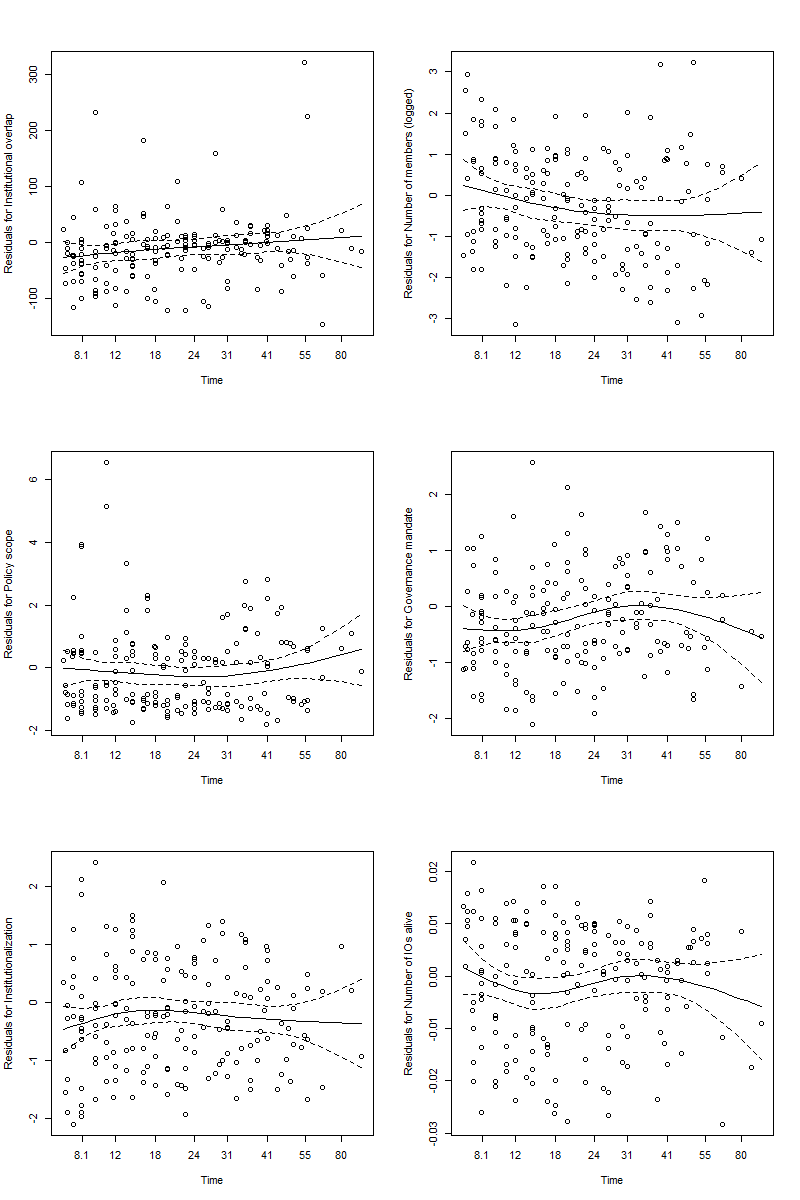
\includegraphics[width=\textwidth]{figuras/schoenfeld2.png}
  \label{fig:schoenfeld}
\end{figure}

\newpage

\section*{Table A5: Results from Table 1 using the Breslow method for ties}
\addcontentsline{toc}{section}{Table A5: Results from Table 1 using the Breslow method for ties}

\begin{table}[H] \centering 
\footnotesize
\begin{tabular}{@{\extracolsep{5pt}}lc} 
\\[-1.8ex]\hline 
\hline \\[-1.8ex] 
 & \multicolumn{1}{c}{\textit{Dependent variable:}} \\ 
\cline{2-2} 
\\[-1.8ex] & IO death \\ 
\hline \\[-1.8ex] 
 Institutional overlap & $-$10.374$^{***}$ \\ 
  & (4.709) \\ 
  & \\ 
 Number of members (logged) & $-$0.275$^{***}$ \\ 
  & (0.101) \\ 
  & \\ 
 Policy scope & $-$0.131 \\ 
  & (0.094) \\ 
  & \\ 
 Governance mandate & $-$0.751$^{***}$ \\ 
  & (0.267) \\ 
  & \\ 
 Governance mandate * ln(t) & 0.170$^{**}$ \\ 
  & (0.085) \\ 
  & \\ 
 Institutionalization & $-$0.233$^{***}$ \\ 
  & (0.063) \\ 
  & \\ 
 Number of IOs alive & $-$0.001$^{*}$ \\ 
  & (0.001) \\ 
  & \\ 
\hline \\[-1.8ex] 
Number of failures & 181 \\ 
Observations & 18,213 \\ 
Log Likelihood & $-$978.683 \\ 
Wald Test & 107.320$^{***}$ (df = 7) \\ 
LR Test & 109.308$^{***}$ (df = 7) \\ 
Score (Logrank) Test & 99.168$^{***}$ (df = 7) \\ 
\hline 
\hline \\[-1.8ex] 
\textit{Note:}  & \multicolumn{1}{r}{$^{*}$p$<$0.1; $^{**}$p$<$0.05; $^{***}$p$<$0.01} \\ 
\end{tabular} 
\end{table} 

\newpage

\section*{Table A6: Results from Table 2 using the Breslow method for ties}
\addcontentsline{toc}{section}{Table A6: Results from Table 2 using the Breslow method for ties}


\begin{table}[H] 
\centering 
\footnotesize
\label{tab:combined_risks} 
\begin{tabular}{@{\extracolsep{5pt}}lcccccc} 
\\[-1.8ex]\hline 
\hline \\[-1.8ex] 
 & \multicolumn{6}{c}{\textit{Dependent variable}} \\ 
\cline{2-7} 
\\[-1.8ex] 
 & \multicolumn{2}{c}{Contract} & \multicolumn{2}{c}{Transformation} & \multicolumn{2}{c}{Inertia} \\ 
\cline{2-3} \cline{4-5} \cline{6-7} 
\\[-1.8ex] 
 & CSH & FG & CSH & FG & CSH & FG \\ 
\\[-1.8ex] 
\hline \\[-1.8ex] 
Institutional overlap & $-$26.516$^{***}$ & $-$23.220$^{**}$ & $-$10.542$^{*}$ & $-$7.333 & $-$2.733 & 1.506 \\ 
 & (11.266) & (11.157) & (7.319) & (7.212) & (8.341) & (8.124) \\ 
Number of members (logged) & $-$0.210 & $-$0.136 & $-$0.138 & $-$0.105 & $-$0.492$^{**}$ & $-$0.444$^{**}$ \\  
 & (0.197) & (0.196) & (0.149) & (0.149) & (0.242) & (0.243) \\ 
Policy scope  & $-$0.250 & $-$0.266 & $-$1.540$^{**}$ & $-$0.547$^{**}$ & $-$0.177 & $-$0.137 \\ 
 & (0.211) & (0.210) & (0.696) & (0.268) & (0.228) & (0.223) \\ 
Policy scope * ln(t) &  &  & 0.452$^{**}$ & 0.015$^{**}$ &  & \\ 
 &  &  & (0.215) & (0.008) &  & \\ 
Governance mandate & $-$0.288$^{**}$ & $-$0.242$^{*}$ & $-$0.142 & $-$0.249 & $-$0.310$^{**}$ & $-$0.263$^{**}$ \\ 
 & (0.141) & (0.138) & (0.096) & (0.161) & (0.162) & (0.159) \\ 
Governance mandate * ln(t) &  &  &  & 0.005 &  & \\ 
 &  &  &  & (0.005) &  & \\ 
Institutionalization & $-$0.264$^{*}$ & $-$0.233$^{*}$ & $-$0.166 & $-$0.124 & $-$0.348$^{**}$ & $-$0.308$^{**}$ \\ 
 & (0.130) & (0.124) & (0.096) & (0.093) & (0.146) & (0.139) \\ 
Number of IOs alive & $-$0.003$^{**}$ & $-$0.003$^{*}$ & $-$0.001 & 0.00001 & $-$0.003 & $-$0.002 \\ 
 & (0.002) & (0.002) & (0.001) & (0.001) & (0.002) & (0.002) \\ 
\hline \\[-1.8ex] 
Number of failures & 46 & 46 & 77 & 77 & 36 & 36 \\ 
Observations & 17,865 & 19,763 & 17,865 & 19,351 & 17,865 & 19,479 \\ 
Log Likelihood & $-$233.115 & $-$244.751 & $-$423.428 & $-$433.861 & $-$186.005 & $-$195.368 \\ 
Wald Test & 54.040$^{***}$ & 40.500$^{***}$ & 30.710$^{***}$ & 26.030$^{***}$ & 63.650$^{***}$ & 47.760$^{***}$ \\ 
\hline 
\hline \\[-1.8ex] 
\multicolumn{7}{l}{\textit{Note:} $^{*}$p$<$0.1; $^{**}$p$<$0.05; $^{***}$p$<$0.01} \\ 
\multicolumn{7}{l}{CSH: Cause-Specific hazards model; FG: Fine-Gray subdistribution hazards model} \\ 
\end{tabular} 
\end{table}

\newpage
\section*{Figure A2: Conditional linear coefficient for Governance mandate}
\addcontentsline{toc}{section}{Figure A2: Conditional linear coefficient for Governance mandate}

\begin{figure}[H]
  \centering
  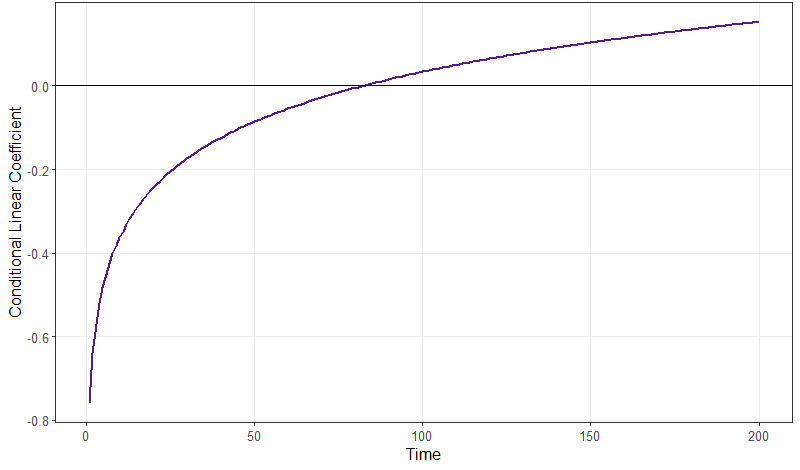
\includegraphics[width=\textwidth]{figuras/condlinearcoef.png}
  \label{fig:condlinearcoef}
\end{figure}

As Flores (\citeyear{flores2022survival}) notes, after correcting the model with the time interaction, multiple quantities of interest can be reported. One possibility is looking at the term $Z\beta_1 + \ln(t)Z\beta_2$ in $\lambda_0(t) \exp\left(Z\beta_1 + \ln(t)Z\beta_2\right)$ . Here, changes in Z reflect changes in the hazard rates. If Z is continuous, the marginal effect of Z on $Z\beta_1 + \ln(t)Z\beta_2$ is: 

\begin{equation*}
\frac{\partial (Z\beta_1 + \ln(t)Z\beta_2)}{\partial Z} = \beta_1 + \beta_2\ln(t)
\end{equation*}

This quantity is the conditional linear coefficient. In the case of the governance mandate dimension of my model, the conditional linear coefficient is $-0.761 + 0.172ln(t)$, where t represents time. Starting from -0.761 at t = 0,  the effect gradually weakens (becomes less negative) over time. Around 84 years ($e^{\frac{0.761}{0.172}}$), the effect is indistinguishable from zero. Therefore, the protective effect of governance mandate in IO survival is relevant in the early stages of an IO, but tends to decrease monotonically and logarithmically over time. 

However, as mentioned, this quantity makes more sense when the variable is continuous. The way I measured governance mandates is discrete. In this case, we should focus on simulated first differences instead.  


\newpage
\section*{Figure A3: Simulated first differences for Governance mandate}
\addcontentsline{toc}{section}{Figure A3: Simulated first differences for Governance mandate}

\begin{figure}[H]
  \centering
  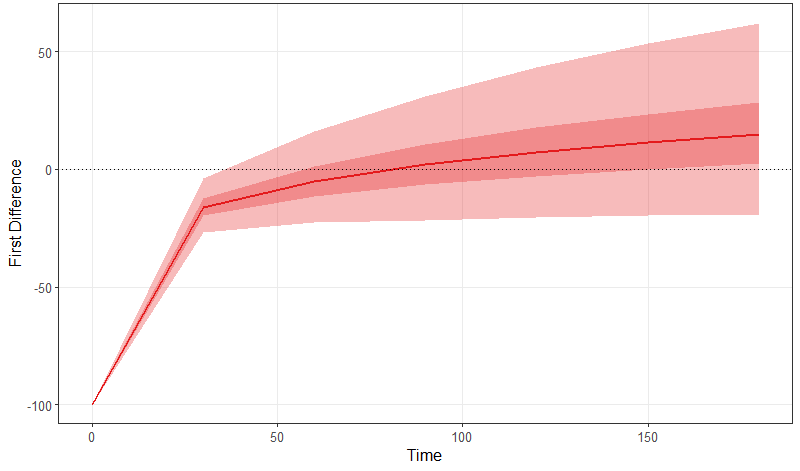
\includegraphics[width=\textwidth]{figuras/simfirstdiff.png}
  \label{fig:simfirstdiff}
\end{figure}

In the case of discrete variables, two quantities of interest are the relative hazards and the first differences, which are the percent changes in the hazard rates (\cite{flores2022survival}). A relative hazard is a type of hazard ratio, and in the context of nonproportionality, it is the following:

\begin{equation*}
\frac{\lambda_i(t)}{\lambda_{\neg i}(t)} = \frac{\lambda_0(t)\exp(Z_i\beta_1 + \ln(t)Z_i\beta_2)}{\lambda_0(t)\exp(Z_{\neg i}\beta_1 + \ln(t)Z_{\neg i}\beta_2)} = \exp((Z_i - Z_{\neg i})(\beta_1 + \ln(t)\beta_2))
\end{equation*}

In this case, the percentual change in the hazard rate for unit i relative to unit $\neg i$ is calculated as follows:

\begin{equation*}
\%\Delta\lambda_i(t) = (\exp((Z_i - Z_{\neg i})(\beta_1 + \ln(t)\beta_2)) - 1) \times 100
\end{equation*}

Figure A3 shows precisely that, i.e., the percent change in the hazard rate as given by a change in my variable Governance mandate. These results confirm what was shown in the previous figure. Here, governance tasks have a time-dependent effect, which has a protective effect on the early stages of an IO’s life cycle, but when time passes, it converges toward zero. 

\newpage

\section*{Table A7: Cox regression with a shared frailty on function}
\addcontentsline{toc}{section}{Table A7: Cox regression with a shared frailty on function}

\begin{table}[H] 
\centering 
\footnotesize
\begin{tabular}{@{\extracolsep{5pt}}lc} 
\\[-1.8ex]\hline 
\hline \\[-1.8ex] 
 & \multicolumn{1}{c}{\textit{Dependent variable: IO death}} \\ 
\hline \\[-1.8ex] 
\textbf{Fixed Effects} &  \\ 
Institutional overlap & $-$9.744$^{**}$ \\ 
  & (4.720) \\ 
  & \\ 
Number of members (logged) & $-$0.264$^{***}$ \\ 
  & (0.100) \\ 
  & \\ 
Policy scope & $-$0.144 \\ 
  & (0.095) \\ 
  & \\ 
Governance mandate & $-$0.775$^{***}$ \\ 
  & (0.267) \\ 
  & \\ 
Governance mandate * ln(t) & 0.175$^{**}$ \\ 
  & (0.085) \\ 
  & \\ 
Institutionalization & $-$0.238$^{***}$ \\ 
  & (0.063) \\ 
  & \\ 
Number of IOs alive & $-$0.002$^{*}$ \\ 
  & (0.001) \\ 
  & \\ 
\hline \\[-1.8ex] 
\textbf{Random Effects} &  \\ 
Variance & 0.042 \\ 
Standard Deviation & 0.205 \\ 
\hline \\[-1.8ex] 
Observations & 18,213 \\ 
Number of failures & 181 \\ 
Integrated Log Likelihood & 113.0 \\ 
Penalized Log Likelihood & 118.7 \\ 
\hline 
\hline \\[-1.8ex] 
\textit{Note:} & \multicolumn{1}{r}{$^{*}$p$<$0.1; $^{**}$p$<$0.05; $^{***}$p$<$0.01} \\ 
\end{tabular} 
\end{table} 

\section*{Table A8: Cox regression with a shared frailty on scope}
\addcontentsline{toc}{section}{Table A8: Cox regression with a shared frailty on scope}

\begin{table}[H] 
\centering 
\footnotesize
\label{tab:coxme_model} 
\begin{tabular}{@{\extracolsep{5pt}}lc} 
\\[-1.8ex]\hline 
\hline \\[-1.8ex] 
 & \multicolumn{1}{c}{\textit{Dependent variable: IO death}} \\ 
\hline \\[-1.8ex] 
\textbf{Fixed Effects} &  \\ 
Institutional overlap & $-$10.54$^{**}$ \\ 
  & (4.711) \\ 
  & \\ 
Number of members (logged) & $-$0.277$^{**}$ \\ 
  & (0.100) \\ 
  & \\ 
Policy scope & $-$0.131 \\ 
  & (0.094) \\ 
  & \\ 
Governance mandate & $-$0.761$^{***}$ \\ 
  & (0.267) \\ 
  & \\ 
Governance mandate * ln(t) & 0.172$^{**}$ \\ 
  & (0.085) \\ 
  & \\ 
Institutionalization & $-$0.236$^{***}$ \\ 
  & (0.063) \\ 
  & \\ 
Number of IOs alive & $-$0.001$^{*}$ \\ 
  & (0.001) \\ 
  & \\ 
\hline \\[-1.8ex] 
\textbf{Random Effects} &  \\ 
Variance & 0.0003992 \\ 
Standard Deviation & 0.01998 \\ 
\hline \\[-1.8ex] 
Observations & 18,213 \\ 
Number of failures & 181 \\ 
Integrated Log Likelihood & 95.16 \\ 
Penalized Log Likelihood & 97.16 \\ 
\hline 
\hline \\[-1.8ex] 
\textit{Note:} & \multicolumn{1}{r}{$^{*}$p$<$0.1; $^{**}$p$<$0.05; $^{***}$p$<$0.01} \\ 
\end{tabular} 
\end{table} 

\section*{Table A9: Cox regression with a shared frailty on region}
\addcontentsline{toc}{section}{Table A9: Cox regression with a shared frailty on region}

\begin{table}[H] 
\centering 
\footnotesize
\label{tab:coxme_model} 
\begin{tabular}{@{\extracolsep{5pt}}lc} 
\\[-1.8ex]\hline 
\hline \\[-1.8ex] 
 & \multicolumn{1}{c}{\textit{Dependent variable: IO death}} \\ 
\hline \\[-1.8ex] 
\textbf{Fixed Effects} &  \\ 
Institutional overlap & $-$9.998$^{**}$ \\ 
  & (4.752) \\ 
  & \\ 
Number of members (logged) & $-$0.220$^{**}$ \\ 
  & (0.106) \\ 
  & \\ 
Policy scope & $-$0.127 \\ 
  & (0.094) \\ 
  & \\ 
Governance mandate & $-$0.778$^{***}$ \\ 
  & (0.268) \\ 
  & \\ 
Governance mandate * ln(t) & 0.176$^{**}$ \\ 
  & (0.085) \\ 
  & \\ 
Institutionalization & $-$0.240$^{***}$ \\ 
  & (0.063) \\ 
  & \\ 
Number of IOs alive & $-$0.002$^{*}$ \\ 
  & (0.001) \\ 
  & \\ 
\hline \\[-1.8ex] 
\textbf{Random Effects} &  \\  
Variance & 0.0314 \\ 
Standard Deviation & 0.177 \\ 
\hline \\[-1.8ex] 
Observations & 18,213 \\ 
Number of failures & 181 \\ 
Integrated Log Likelihood & 111.7 \\ 
Penalized Log Likelihood & 117.5 \\ 
\hline 
\hline \\[-1.8ex] 
\textit{Note:} & \multicolumn{1}{r}{$^{*}$p$<$0.1; $^{**}$p$<$0.05; $^{***}$p$<$0.01} \\ 
\end{tabular} 
\end{table} 


\section*{Table A10: Cox regression with a shared frailty on membership format}
\addcontentsline{toc}{section}{Table A10: Cox regression with a shared frailty on membership format}

\begin{table}[H] 
\centering 
\footnotesize
\label{tab:coxme_model} 
\begin{tabular}{@{\extracolsep{5pt}}lc} 
\\[-1.8ex]\hline 
\hline \\[-1.8ex] 
 & \multicolumn{1}{c}{\textit{Dependent variable: IO death}} \\ 
\hline \\[-1.8ex] 
\textbf{Fixed Effects} &  \\ 
Institutional overlap & $-$10.977$^{*}$ \\ 
  & (4.800) \\ 
  & \\ 
Number of members (logged) & $-$0.229$^{**}$ \\ 
  & (0.105) \\ 
  & \\ 
Policy scope & $-$0.117 \\ 
  & (0.093) \\ 
  & \\ 
Governance mandate & $-$0.259$^{***}$ \\ 
  & (0.068) \\ 
  & \\ 
Institutionalization & $-$0.252$^{***}$ \\ 
  & (0.065) \\ 
  & \\ 
Number of IOs alive & $-$0.001$^{*}$ \\ 
  & (0.001) \\ 
  & \\ 
\hline \\[-1.8ex] 
\textbf{Random Effects} &  \\ 
Variance & 0.000079 \\ 
Standard Deviation & 0.009 \\ 
\hline \\[-1.8ex] 
Observations & 17,822 \\ 
Number of failures & 178 \\ 
Integrated Log Likelihood & 106.2 \\ 
Penalized Log Likelihood & 106.2 \\ 
\hline 
\hline \\[-1.8ex] 
\textit{Note:} & \multicolumn{1}{r}{$^{*}$p$<$0.1; $^{**}$p$<$0.05; $^{***}$p$<$0.01} \\ 
\end{tabular} 
\end{table}

\newpage

\printbibliography

\end{document}